%\VignetteIndexEntry{TapeR: Felxible stem taper modelling}
\documentclass[english,11pt]{article}
%\documentclass[a4paper,11pt]{article}
\usepackage[a4paper]{geometry}
\geometry{verbose,tmargin=2cm,bmargin=2cm,lmargin=2cm,rmargin=2cm,footskip=1cm}

\usepackage{Sweave}
\usepackage{color}
\usepackage{graphicx}
\usepackage{booktabs}
\usepackage[authoryear]{natbib}
\usepackage{url}
\usepackage[utf8]{inputenc}

% \setlength{\oddsidemargin}{1cm}
% \setlength{\textwidth}{15cm}
% \setlength{\topmargin}{-2.2cm}
% \setlength{\textheight}{22cm}

% \usepackage{amssymb}
% \usepackage{amsmath}


%\usepackage{hyperref}
\usepackage[linkcolor=blue, bookmarks=true, citecolor=blue, colorlinks=true, linktocpage, a4paper]{hyperref}



\title{TapeR: Flexible stem taper modelling}
\author{Edgar Kublin\thanks{Forest Research Institute of
    Baden-W{\"u}rttemberg, Freiburg, Germany}, Johannes Breidenbach\thanks{Norwegian Institute of Bioeconomy Research, 1431 {\AA}s, Norway, job@nibio.no}}
%%\date{}
%\address{Norwegian Institute for Forest and Landscape}

\begin{document}
\Sconcordance{concordance:TapeR.tex:TapeR.Rnw:%
1 46 1 1 2 4 0 1 2 3 1 1 2 4 0 1 2 1 1 1 2 4 0 1 2 16 1 1 4 2 0 1 3 1 0 %
2 1 1 3 1 0 1 5 2 0 2 1 1 4 2 0 1 5 8 0 1 3 12 1}

\maketitle

%\tableofcontents


\section{Introduction}
The \texttt{TapeR} package implements methods described in \citep{kublin2013}.

If \texttt{R} is running, the \texttt{TapeR} package can be installed
by typing

\begin{Schunk}
\begin{Sinput}
> install.packages("TapeR")
\end{Sinput}
\end{Schunk}
into the console\footnote{The character "\texttt{>}" is not
  part of the command. A working Internet connection is required.}.

The command
\begin{Schunk}
\begin{Sinput}
> library(TapeR)
\end{Sinput}
\end{Schunk}
loads the package into the current workspace. We can get an overview of
the packages' contents by typing
\begin{Schunk}
\begin{Sinput}
> ?TapeR
\end{Sinput}
\end{Schunk}

\section{Using the TapeR functions}

\subsection{Fitting a taper model}

A taper model can be fit to measured pairs of diameter and
corresponding heights. Typically, those data are recorded for regular stem sections but
the data can also be availabe at irregular distances. Important is for
the method implemented in this packages is
that the stem height is available too. We will load some example data
and fit a taper model. Note that in real applications, the dataset must be
considerably bigger in order to provide reliable taper models that are
valid over larger spatial extents. For example, the data set
\texttt{SK.par.lme} provides the taper model parameters
based on 338 Norway spruce trees in Germany.


\begin{Schunk}
\begin{Sinput}
> #load example data
> data(DxHx.df)
> #prepare the data (could be defined in the function directly)
> Id = DxHx.df[,"Id"]
> x = DxHx.df[,"Hx"]/DxHx.df[,"Ht"]#calculate relative heights
> y = DxHx.df[,"Dx"]
> #plot the example data
> plot(x,y,pch=as.character(Id),xlab="Relative height (m)", ylab="Diameter (cm)")
> #define the relative knot positions and order of splines
> 
> knt_x = c(0.0, 0.1, 0.75, 1.0) # B-Spline knots: fix effects
> ord_x = 4 # ord = order (4 = cubic)
> knt_z = c(0.0, 0.1, 1.0); ord_z = 4 # B-Spline knots: rnd effects
> #fit the model
> taper.model <- TapeR_FIT_LME.f(Id, x, y, knt_x, ord_x, knt_z, ord_z,
+ IdKOVb = "pdSymm")
> #save model parameters for documentation or dissimination
> #parameters can be load()-ed and used to predict the taper
> #or volume using one or several measured dbh
> spruce.taper.pars <- taper.model$par.lme
> #save(spruce.taper.pars, file="spruce.taper.pars.rdata")##uncomment to save
\end{Sinput}
\end{Schunk}
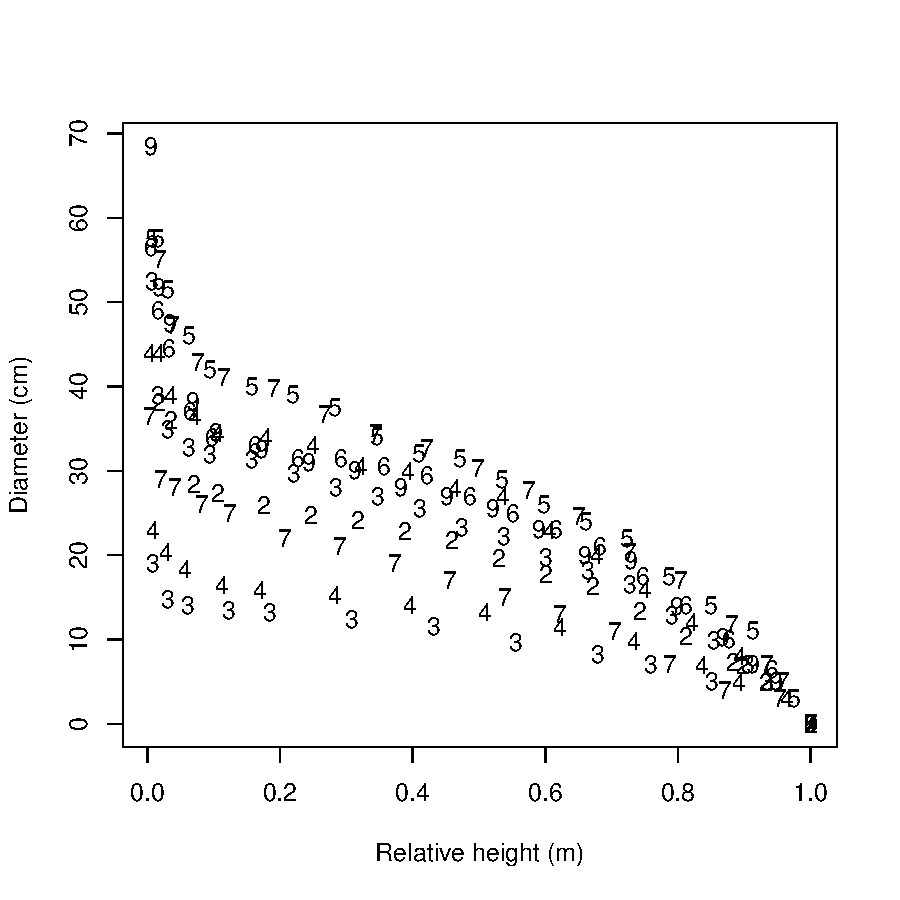
\includegraphics{TapeR-004}


\begin{thebibliography}{---}
\bibitem[Kublin et al.(2013)]{kublin2013} Kublin, E., Breidenbach, J.,
  K{\"a}ndler, G. (2013): \emph{A flexible stem taper
  and volume prediction method based on mixed-effects B-spline
  regression}. Eur J For Res, 132:983-997.
%
\end{thebibliography}


\end{document}

